\subsubsection{Distribution of nodes: Graph coloring}
In order to implement a parallel asynchronous version of the Tutte algorithm, it is necessary to separate graph nodes into different sets. The objective is to extract an independence between nodes. In fact, each node has to move while the neighbours maintain their positions. Thus, the independence must be between the moving node and its neighbours. This problem is similar to the famous problem of graph coloring.
\paragraph*{}
The objective of the modified Tutte algorithm is to handle graphs of thousands of nodes. To separate such a number of nodes, it is more effective to use a heuristic of the algorithm of graph coloring.\\
The greedy algorithm is a simple and good solution to separate nodes into sets fast and effectively.~\cite{pf}
\paragraph*{}
The algorithm used in this project is :
\begin{verbatim}
G={V,E}
Y = V
color = 0
While Y is not empty
   Z = Y
   While Z is not empty
      Choose a node v from Z
      Colorate v with color
      Y = Y - v
      Z = Z - v - {neighbors of v}
   End while
   color ++
End while
\end{verbatim}

This algorithm is known to use at most $d(G)+1$ colors where $d(G)$ represents the largest value of the degree in the graph G. However, its shortcoming is that it produces sets of different size. This can be inconvenient for task distribution.
\subsubsection{Applying Tutte algorithm to sets}
Once a set of nodes is obtained, it is possible to apply a parallel Tutte algorithm. The question is how to parallelize it on sets of nodes. The natural idea is to attribute one set per thread :
\begin{figure}[!h]
\centering
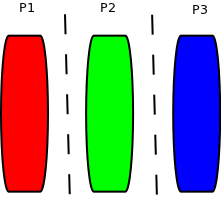
\includegraphics[scale=0.5]{img/distribution_verticale.png}
\caption{One set per thread}
\end{figure}
This distribution is far from being optimal. In fact, each thread has to lock the neighbours nodes before moving the concerned node, which introduces an important critical section. In addition to being unfair, this distribution is limited by the number of sets produced.\\

The best distribution for sets obtained by graph coloring is to execute $n$ threads on one set. Each thread moves a number of nodes of the set without any critical section, since each node of the set is not the neighbour of all the other nodes of the same set. Once the thread has moved all its nodes of the set, it must wait for other threads to have completed the same process (implemented by a barrier). Then, the overall process is applied to the next set.

\begin{figure}[!h]
\centering
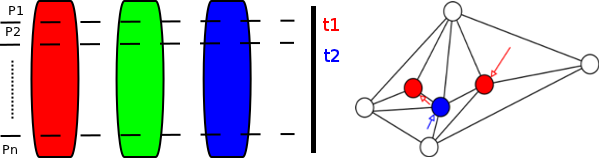
\includegraphics[scale=0.5]{img/distrib.png}
\caption{$n$ threads per set}
\end{figure}



